
\section{Evaluation}

We ran our system on the web at large, attempting to discover \ehi
vulnerabilities in web applications. We used as a seed to
\texttt{Crawler} the Alexa top 10,000 websites as well as a feed of
10,000 random blog pings per day from \url{weblogs.com}. All domains
were crawled to a maximum depth of four, and the crawler respected the
\texttt{robots.txt} directive. This seed enabled \texttt{Crawler} to
get an overview of not only the popular websites (from the Alexa top
10k) but also the long-tail of blog posts and websites that they
linked to.


From our extensive crawl of the web, we were able to gather the data
shown in Table~\ref{tab:data}. We ran the system for 76 days, during which our system crawled \urls unique URLs,
and found a total of \forms\ forms from \uniqueforms\ unique domains. Out of these forms, our system
found \emailforms\ forms that contained an \email field, from \uniqueemailforms\ unique domains.
Table~\ref{tab:fuzzed_data} shows the quantity of \emails we received for the benign and malicious payloads. 
\begin{table}[tbp]
	\centering
	\scriptsize
	\begin{tabular}{|c|c|}
		\hline
		\multicolumn{1}{|c|}{\textbf{Type of Data}} &
		\multicolumn{1}{c|}{\textbf{Quantity}}\\
		\hline
		URLs Crawled & \urls \\
		\hline
		Total Forms found & \forms \\
		\hline
		Forms with E-Mail Fields & \emailforms \\
		\hline
	\end{tabular}
	\caption[\titlecap{Collected data}]{The data collected for our
      project.}
    \vspace{-5ex}
	\label{tab:data}
\end{table}

\begin{table}[tbp]
	\centering
	\scriptsize
	\begin{tabular}{|c|c|c|}
		\hline
		\multicolumn{1}{|c|}{\textbf{Type of fuzzing}} &
		\multicolumn{1}{c|}{\textbf{Forms fuzzed}} &
		\multicolumn{1}{c|}{\textbf{E-Mails received}}\\
		\hline
		Regular payload & \fuzzed & \recd \\
		\hline
		Malicious payload & \malfuzzed & \success \\
		\hline
	\end{tabular}
	\caption[\titlecap{Fuzzed data}]{The data we fuzzed and the e-mails we received.}
    \vspace{-5ex}    
	\label{tab:fuzzed_data}
\end{table}


\noindent\textbf{\Email received from forms.} The \emails that we
received can be categorized into two categories. (1) \Emails due to
regular payload: This represents the total number of web applications
that sent \emails to us. This indicates that we were able to
successfully submit the forms on these sites to trigger the web
application to send an \email. (2) \Emails due to malicious payload:
Once we receive an \email from a web application due to the regular
payload, we fuzz those forms with the malicious payloads. This field
represents the total number of unique URLs that contain an \ehi
vulnerability.


%%Table~\ref{tab:fuzzed_data} shows the quantity of \emails that we received for the benign and malicious payloads. 
%\begin{table}[tbp]
	\centering
	\scriptsize
	\begin{tabular}{|c|c|c|}
		\hline
		\multicolumn{1}{|c|}{\textbf{Type of fuzzing}} &
		\multicolumn{1}{c|}{\textbf{Forms fuzzed}} &
		\multicolumn{1}{c|}{\textbf{E-Mails received}}\\
		\hline
		Regular payload & \fuzzed & \recd \\
		\hline
		Malicious payload & \malfuzzed & \success \\
		\hline
	\end{tabular}
	\caption[\titlecap{Fuzzed data}]{The data we fuzzed and the e-mails we received.}
    \vspace{-5ex}    
	\label{tab:fuzzed_data}
\end{table}

%
%\noindent\textbf{\Email received from forms.} The \emails that we
%received can be categorized into two categories. (1) \Emails due to
%regular payload: This represents the total number of web applications
%that sent \emails to us. This indicates that we were able to
%successfully submit the forms on these sites to trigger the web
%application to send an \email. (2) \Emails due to malicious payload:
%Once we receive an \email from a web application due to the regular
%payload, we fuzz those forms with the malicious payloads. This field
%represents the total number of unique URLs that are contain an \ehi
%vulnerability.


\subsection{Analysis of the Received \Email Data}

During our analysis of the received \emails, we found that the \emails that we received belonged to three categories:

(1) \Emails with the \texttt{bcc} header successfully injected. This form
of injection was our initial objective, and we found
% Adam: Sai, why isn't this number a command? - DONE.
\ehibcc such \emails in our received \emails. This validates that the
web applications that sent these \emails are vulnerable to \ehi.
	
(2) \Emails with the \texttt{To} header successfully injected. We
discovered an unintended vulnerability class during our analysis,
which we call \texttt{To~header injection}. These injections reflect
the ability to inject any number of \email addresses into the
\texttt{to} field of the SMTP message while being unable to inject any
other header into the \emails. We found \ehito such \emails in our
received \emails. We attribute this behavior to inconsistent
sanitization by the application.
   
While not allowing us complete control over content of the \emails
sent, \texttt{To header injection} makes it possible to append any
number of \email addresses, thereby enabling us to leak information or
perform DoS (Denial of Service) attacks against the web application.
	
(3) \Emails with the \texttt{x-check} header successfully injected. The
third category of \emails received were \emails with the
\texttt{x-check} header injected. As discussed in
Section~\ref{analyze:detect_x_check}, we can differentiate between
unsuccessful attempts and successful attempts by injecting the
additional header and checking whether headers other than the
\texttt{bcc} header can be injected into the generated \email.
\ehixcheck \emails were received with the \texttt{x-check} header
injected.

% Adam: Sai, we need to put the actual numbers in the text. We cannot count on the readers to look at the table (of course, we should use the commands
We list each category and the number of \emails received by that
category in Table~\ref{tab:analysis}. We explain the combination of
these header injections (4-7) as follows:

%\begin{table}[tbp]
\begin{wraptable}{r}{6.5cm}
	\centering
	\scriptsize
    \vspace{-4ex}
	\begin{tabular}{|l|p{1cm}|}
		\hline
		\textbf{Type of Injection} & \textbf{\# e-mails}\\
		\hline
		E-Mail Header Injections with \texttt{bcc} header & \ehibcc \\
		\hline
		E-Mail Header Injections with \texttt{x-check} header & \ehixcheck \\
		\hline
		\texttt{To header} injections alone & \ehito \\
		\hline
		Injections with both \texttt{bcc} and \texttt{x-check} headers & \ehibccxcheck \\
		\hline
		Both \texttt{To header} injections and x-check headers &
		\ehitoxcheck \\
		\hline
		\texttt{x-check} headers found in \texttt{nuser} e-mails & \ehinuserxcheck \\
		\hline
		Unique \texttt{x-check} headers found in \texttt{nuser} e-mails & \ehiuniquenuserxcheck \\
		\hline
		Total successful injections (1 + 3 + 7) & \success \\
		
		\hline
	\end{tabular}
	\caption[\titlecap{Analysis of the data}]{Classification of the e-mails that we received into broad categories of the vulnerability.}
    \vspace{-5ex}
	\label{tab:analysis}
    %\end{table}
\end{wraptable}


\Email Header Injections with both \texttt{bcc} and \texttt{x-check}
headers: These represent the scenario where an attacker can inject
multiple headers into the \emails. We can see that 54\% of the
received \texttt{bcc} header injected \emails are also susceptible to
being injected with additional headers.
      % Adam: What is the exact percentage? We should use that rather than an approximate number - DONE.
	
Both \texttt{To} header injections and \texttt{x-check} headers: This
combination shows us that in addition to being able to inject into the
\texttt{To} fields, we injected additional headers into the \email. It
is not clear what causes this behavior; however, these can be
exploited to achieve the same result as a regular \ehi.
	
Total \texttt{x-check} headers and unique \texttt{x-check} headers
found in \texttt{nuser} \emails: We found a total of \ehinuserxcheck
\emails in the \texttt{nuser} account. Out of these,
\ehiuniquenuserxcheck had unique form ids that were \emph{not} already
found in the \texttt{maluser} account. We attribute these \emails to
(probably) being sent by a web application that was built with Python
or another language having a similar behavior with respect to ignoring
duplicate headers while constructing an \email, thus appending the
\texttt{x-check} header and \emph{not} the \texttt{bcc} header.
      % Adam: What is the actual behavior? This is confusing. - Changed. DONE.
	
Total successful injections: This represents the total number of
successful injections. This includes the \ehi with \texttt{bcc}
header\,(1), \texttt{To} header injections\,(3), and Unique
\texttt{x-check} headers found in \texttt{nuser} \emails\,(7). A total
of \success vulnerabilities were found by our system.

      % Adam: we need the actual #s here too. These are the core results of our analysis, they need to be in the text. - DONE.


\subsection[The Pipeline]{Understanding the Data Pipeline}

%This section serves to represent our pipeline quantitatively and graphically. 
Table~\ref{tab:pipeline} shows the data gathered by our pipeline, with the differential changes at each stage of the pipeline. At each stage of the pipeline, the amount of data decreases, for instance, out of the \urls\ URLs we crawled, only \forms\ forms (\formsDelta) were found. Out of these, only \emailforms\ forms (\emailformsDelta) contained e-mail fields.

In our fuzzing attempts, the same behavior is observed. We fuzzed \fuzzed\ forms with the regular payload, which resulted in a total of \recd\ e-mails~(\recdDelta). After analysis of the received e-mails, we further fuzzed \malfuzzed\ forms, which resulted in \success\ e-mails (\successDelta) which contain the vulnerability across \ips IP addresses from \domains domains.

We attribute the difference in the number of forms found to the number of forms fuzzed (a difference of \diffFoundFuzz forms) to the presence of bot-blocking mechanisms on a website (discussed in Section~\ref{limitations}), though we do not know what percentage was caused by each bot-blocking mechanism discussed in Section~\ref{limitations}. 

Note that over 1\% of the forms that were not fuzzed (100 out of \diffFoundFuzz) were also tested manually using PostMan to generate HTTP requests with payloads to verify that our system was working as intended.

\begin{table}[tbp]
%\begin{wraptable}{r}{7cm}
	\centering
	\scriptsize
	\begin{tabular}{|l|c|c|}
		\hline
		\textbf{Pipeline Stage} & \textbf{Quantity} & \textbf{Differential}\\
		\hline
		Crawled URLs  & \urls & $\Delta$ d2/d1 * 100 \\
		\hline
		Forms found  & \forms & \formsDelta \\
		\hline
		E-Mail Forms found  & \emailforms & \emailformsDelta \\
		\hline
		Fuzzed with regular payload  & \fuzzed & \fuzzedDelta \\
		\hline
		Received e-mails  & \recd & \recdDelta \\
		\hline
		Fuzzed with malicious payload  & \malfuzzed & \malfuzzedDelta \\
		\hline
		Successful attacks  & \success & \successDelta \\
		\hline

	\end{tabular}
	\caption[\titlecap{Data gathered by our pipeline}]{Data gathered
      by our pipeline at each stage}
    
	\label{tab:pipeline}
\end{table}
%\end{wraptable}



% Adam: this is an important part of our contribution, but I don't think that it belongs here. 
%% From our research, it is clear that E-Mail Header Injection is quite widespread as a vulnerability, appearing on \successDelta\ of forms that we were able to perform automated attacks on. This value acts as a lower bound for E-Mail Header Injection vulnerability, and can quite easily be much more if the attacks were of a more concentrated nature, crafted for the individual websites and less automated.

\subsection{Analysis of Vulnerable domains}

We performed the following analyses on the vulnerable domains:
\begin{itemize}
	\item Checking Alexa rankings of the vulnerable domains.
	\item Investigating the back-end languages used by the vulnerable domains.
	\item Analyzing the presence of DKIM (DomainKeys Identified Mail), SPF (Sender Policy Framework), and DMARC (Domain-based Message Authentication, Reporting \& Conformance) mechanisms on these domains.
\end{itemize}


\subsubsection{Alexa rankings of vulnerable domains.}
We searched through the Alexa rankings data\cite{alexa} for the domains that were found to be vulnerable, and found 135 of these domains in the top 1 million ranked websites. A detailed distribution of the rankings is shown in Table~\ref{tab:alexa} / Figure~\ref{fig:alexa_data_bar} / Figure~\ref{fig:alexa_data_pie}.

%TODO Adam: Need to decide if table or graph, if graph, then Pie vs Bar.
%\begin{table}[tbp]
%	\centering
%	\scriptsize
%	\begin{tabular}{|l|c|}
%		\hline
%		\textbf{Alexa Ranking Ranges} & \textbf{Vulnerable domains} \\
%		\hline
%		0-5K & 1 \\
%		\hline
%		5-50k & 7 \\
%		\hline
%		50k-100k & 6 \\
%		\hline
%		100k-250k & 23 \\
%		\hline
%		250k-500k & 30 \\
%		\hline
%		500k-1m & 68 \\
%		\hline		
%	\end{tabular}
%	\caption[\titlecap{Distribution of vulnerable domains based on Alexa Rankings}]{Distribution of vulnerable domains based on Alexa Rankings}
%	\vspace{-5ex}
%	\label{tab:alexa}
%\end{table}

\begin{figure}
	\centering
	\begin{minipage}{.5\textwidth}
		\centering
		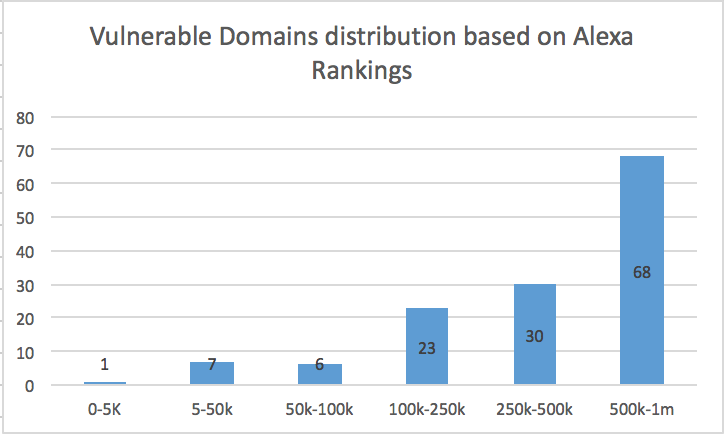
\includegraphics[width=.95\linewidth]{alexa_data_bar}
		\captionof{figure}{Distribution of vulnerable domains based on Alexa Rankings}
		\label{fig:alexa_data_bar}
	\end{minipage}%
	\begin{minipage}{.5\textwidth}
		\centering
		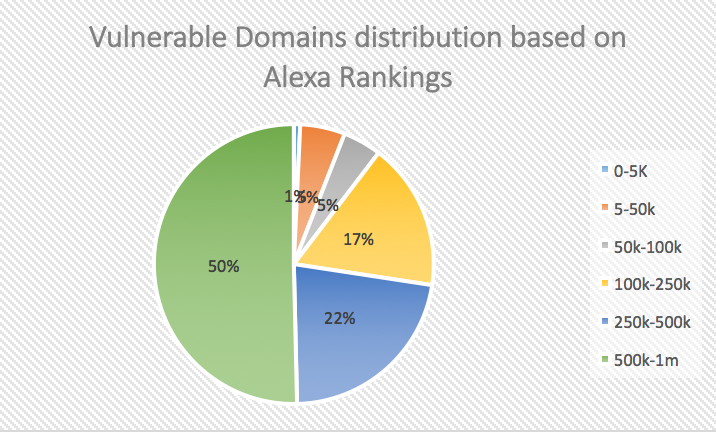
\includegraphics[width=.95\linewidth]{alexa_data_pie}
		\captionof{figure}{Distribution of vulnerable domains based on Alexa Rankings}
		\label{fig:alexa_data_pie}
	\end{minipage}
	\vspace{-1.5ex}
\end{figure}


%TODO Adam: Is a table/graph for backend technologies needed?
% apparently \subsubsection need to have a period at the end.
\subsubsection{Back-end technologies of vulnerable domains.}
We investigated the top 100 vulnerable domains on our list (based on the alexa rankings) to find the back-end technologies used by these vulnerable domains to see if there was any recurring pattern. Using BuiltWith~\cite{builtwith} and wappalyzer~\cite{wappalyzer}, we found that a majority of the vulnerable domains (79\%) used PHP as one of the back-end technologies, while 17\% of domains used WordPress and another 14\% used ASP.Net. Other technologies used include Java (5\%), Ruby on Rails (1\%), and Perl (1\%). We also found a combination of other technologies like Magento, CakePHP, CodeIgniter, Joomla, mail.ru and Drupal being used in conjunction with one of the above languages. A point to be noted is that 4\% of the websites also used Contact Form 7~\cite{CF7}, which is supposed to protect against such attacks. 

\subsubsection{Presence of e-mail spoofing protection on vulnerable domains.}
\subsection{Exploitation Evidence}

We compared the \ips IPs that our system found to be vulnerable to \ehi against 13 well-known IP blacklists, to see if these IPs were being exploited by attackers to send spam. The blacklists that we used were: 
\texttt{zen.spamhaus.org},
\texttt{spam.abuse.ch},
\texttt{cbl.abuseat.org},
\texttt{virbl.dnsbl.bit.nl},
\texttt{dnsbl.inps.de},
\texttt{ix.dnsbl.manitu.net},
\texttt{dnsbl.sorbs.net},
\texttt{bl.spamcannibal.org},
\texttt{bl.spamcop.net},
\texttt{dnsbl-1.uceprotect.net},
\texttt{dnsbl-2.uceprotect.net},
\texttt{dnsbl-3.uceprotect.net},
\texttt{db.wpbl.info}.

We found that \ipsblacklist of these IPs were blacklisted on at least one of the above blacklists for sending out spam, and \ipsblacklistmulti of them were found on multiple blacklists. We do not have enough data to make an observation about whether these attackers are exploiting \ehi to send out the spam, as an alternative hypothesis is that these IPs are on the blacklists because the server has different vulnerabilities that attackers exploit to cause the server to send spam (assuming that the server is normally benign).  

\subsection{Emails with Malicious Attachments}
As additional analysis to find domains on the internet that send out malicious attachments, we checked the \emails received by the `reguser' account (which are injected with regular \email addresses and not malicious data) for the presence of attachments that may contain malicious software, which will indicate that the server itself is not benign. 

To do this, we passed the \totalattachmentcount attachments we received to VirusTotal~\cite{virustotal} -- an online malware scanner that checks for the presence of malware by running 40+ virus scanners on the uploaded files. We found that out of the \totalattachmentcount attachments, \totalvirusemails were malicious, out of which \totalvirusattachmentcount were from unique domains. This data is just a by-product of our research and could very well lead to future research.
%It is to be noted that none of these domains were found on the spam analysis we did earlier, indicating that if these could be exploited, we could send emails with malicious attachments to other people using these servers.

\subsection{Responsible Disclosure of Discovered Vulnerabilities}
After we discovered an \ehi vulnerability on a particular website, we attempted to notify the developers of the vulnerable web application, along with a brief description of the vulnerability.
We chose to \email the following mailboxes, following the rules
specified in RFC~2142~\cite{rfc2142}: \texttt{security@domain.com},
\texttt{admin@domain.com}, and \texttt{webmaster@domain.com}
 
Out of the \domains\ vulnerable domains found, only
\emailedDefaultmailbox websites had the mailboxes able to receive
\emails. For the remaining domains, we used the
\texttt{whois}~\cite{whois} data to find the contact details of the
owner and then \emailed them. We received \responses developer
responses, confirming \confirmed discovered vulnerabilities. Four of
the developers fixed the vulnerability on their website.

From our research, it is clear that \ehi is quite widespread as a
vulnerability, appearing on \successDelta\ of forms that we were able
to perform automated attacks on. This value acts as a \emph{lower
  bound} for prevalence of \ehi vulnerability, and can quite easily be
larger if the attacks were broader, crafted for the individual web
application, and less automated.


%% \begin{table}[tbp]
%% \centering
%% \scriptsize
%% \begin{tabular}{|c|c|c|}
%% 	\hline
%% 	\multicolumn{1}{|p{2cm}}{\centering \textbf{Notified websites}} &
%% 	\multicolumn{1}{|p{2cm}|}{\centering \textbf{Developer Responses}} &
%% 	\multicolumn{1}{p{2cm}|}{\centering \textbf{Confirmed discoveries}}\\
%% 	\hline
%% 	\domains\ & \responses & \confirmed \\
%% 	\hline
%% \end{tabular}
%% 	\caption[\titlecap{}]{Responsible disclosure of the discovered vulnerabilities to developers and the number of received responses.}
%% 	\label{tab:devresp}
%% \end{table}

% Adam: did we get updated notifications? - updated. DONE.

